\chapter{Simulation}
\label{ch:simulation}

Monte Carlo simulation (MC) refers to the practice
of estimating the probability distribution of the outcomes
of a complex and non-deterministic chain of events
by running a (pseudo-random) simulation of the process multiple times
and recording the distribution of the simulated outcomes.
MC is commonly used to estimate detection efficiencies,
a detector's energy response,
and other quantities that have a highly nontrivial dependence
on basic geometric and kinematic quantities.

A distinction is often made between a ``full Monte Carlo''
and a ``toy Monte Carlo.''
In a full MC, each particle is propagated through a series of small time steps,
with various probabilities to interact, decay, deposit energy, and/or be detected,
depending on the material being traversed.
As the name suggests, toy MCs adopt simplifications from the full approach,
and these simplifications can vary widely.
One prototypical example is to use the average $\nicefrac{dE}{dx}$
and a particle's propagation distance
(perhaps determined by drawing from an exponential distribution
based on the decay time and velocity)
to determine the amount of energy deposited by a particle
before it decays.
The simplifications made to toy MCs usually limit their validity
to highly specific scenarios.

Three separate toy MC simulations were used in this analysis
to simulate individual IBD events (\cref{sec:thu_toymc}),
the Daya Bay data stream (\cref{sec:toymc}),
and entire data sets (\cref{sec:lbnl_toymc}).

\section{Individual IBD event simulation}
\label{sec:thu_toymc}

The individual event toy MC was designed
to study detection efficiencies and the detector energy response \cite{nh2016technote}.
Each event began as a \nuebar{} of a given energy interacting via IBD
with an atom in a given region of the Daya Bay AD
(GdLS, LS or acrylic).
The interaction products ($e^+$ and $n$),
were simulated using a full MC implemented using the GEANT4 library \cite{geant4}.
The full simulation included
the positron's energy depositions into the scintillator
and its annihilation,
the neutron's thermalization, scattering, and capture on a nucleus (or escape),
and the resulting $\gamma$ rays' propagation and interactions.
The resulting electrons and positrons from the $\gamma$ ray interactions
were also simulated.
During propagation, an electron could
``deposit'' energy in the liquid scintillator,
escape from the scintillating volume,
or scatter and create another energetic electron.
The total amount of deposited energy was saved as $E_{\text{dep}}$.

To obtain a final simulated reconstructed energy,
a parametrized nonlinearity model and resolution were used
rather than implementing the effects in a full MC.
The scintillator and electronics nonlinearities were applied
to the deposited energy $E_{\text{dep}}$
(see \cref{subsec:abs_energyscale}).
The energy resolution (\cref{subsec:resolution}) used in the MC
was modified to reflect
the absence of detector non-uniformity in the simulation
by setting the $a$ parameter to be 0:
\begin{equation}
    \frac{\sigma_E}{E} = \sqrt{0 + \frac{b^2}{E} + \frac{c^2}{E^2}}
\end{equation}

The simulation was used to generate a data set
where the incident \nuebar{} spectrum
matched the predicted unoscillated reactor \nuebar{} spectrum.
The distributions of simulated prompt and delayed reconstructed energies,
shown in \cref{fig:prompt_eff_mc},
could be used as estimates of the actual distributions.
In other analyses \cite{nh2016}, the MC estimates
for absolute efficiencies of the prompt and delayed energy cuts
were computed from this simulation.
In this analysis, the absolute efficiencies were not used.
However, other quantities based on the simulated quantities
were used.

\begin{figure}
    \centering
    \includegraphics[width=0.49\textwidth]{%
        ch_event_selection/prompt_energy_mc%
    }
    \includegraphics[width=0.49\textwidth]{%
        ch_event_selection/delayed_energy_mc%
    }
    \caption{Spectrum of reconstructed energy for simulated IBD prompt (left)
        and delayed (right) events
        in the Monte Carlo study used to compute the prompt and delayed
        energy cut absolute efficiencies.
        The prompt spectrum is also used to compute the prompt energy cut
    efficiency AD-uncorrelated uncertainty.}
    \label{fig:prompt_eff_mc}
\end{figure}

The first quantity was the correction to the prompt energy cut efficiency
based on the baseline dependence of the oscillation probability
(see \cref{subsec:prompt_energy}).
This correction was computed at a given point in parameter space
(value of \thetaot{}, $\Delta m^2_{32}$, and AD-reactor pair)
by creating a histogram of reconstructed prompt energy
where each entry was weighted by the oscillation probabilty
at the ``true'' \nuebar{} energy saved by the simulation.
The resulting efficiency could be compared
with the nominal efficiency assuming no oscillations.
The relative difference was applied as a correction
during the near-far projection procedure in \cref{subsec:flux_fraction}.

The second quantity produced by the simulation
was the dependence of the prompt energy spectrum and cut efficiency
on changes to the relative energy scale between ADs (see \cref{subsec:rel_energyscale}).
A shift in energy scale was modeled by
creating a histogram of reconstructed prompt energy,
but where the value of the energy was scaled
by the uncertainty of the relative energy scale, \SI{\pm0.5}{\percent}.
The resulting change to the prompt energy cut efficiency, \SI{\pm0.1}{\percent},
is the AD-uncorrelated uncertainty for that efficiency.
Shifting the energy scale also changes the shape of the spectrum,
which was quantified by comparing the change in number of events
in each bin of the histogram with and without the re-scaled energy values.
The oscillation dependence of the spectral shape was also accounted for.

For a particular bin $b$ of reconstructed energy in AD $i$,
the relative energy scale correction $a_{\text{relE},i}^{(b)}$
was defined as the difference in bin content with and without
the relative energy scale shift of \SI{\pm0.5}{\percent},
divided by the bin content without the shift:
\begin{equation}
    a_{\text{relE},i}^{\pm,(b)}(\thetaot, \Delta m^2_{32}) =
    \frac{N^\pm(\thetaot, \Delta m^2_{32}) - N^0(\thetaot, \Delta m^2_{32})}%
    {N^0(\thetaot, \Delta m^2_{32})},
\end{equation}
where the $+$ refers to scaling the energy by \SI[retain-explicit-plus]{+0.5}{\percent}
and the $-$ refers to scaling by \SI{-0.5}{\percent}.
During the fit procedure, the impact of this correction
was controlled by a pull parameter.
The fitter automatically switched between the $+$ and $-$ values
depending on the sign of the pull parameter.

This correction was intentionally not normalized;
the application of $a_{\text{relE},i}^{\pm,(b)}$ to all bins
could change the total number of events.
The impact of the change in total number of events
is equivalent to the previously-mentioned change
to the prompt energy cut efficiency induced by the relative energy scale shift.
To avoid double-counting the change in number of events
due to a shift in relative energy scale,
the prompt energy cut efficiency is omitted
from the fit model and from the constraint
on the pull parameter representing the overall detection efficiency uncertainty.

\section{Data stream simulation}
\label{sec:toymc}

The Daya Bay event selection process (\cref{ch:event_selection})
depends on more than just the properties of a single AD event;
there are anti-correlation requirements such as the muon veto,
and correlation requirements to select only double coincidences.
Additionally, the basis for the determination of the accidental background rate
relies heavily on the accurate extraction of
the rate of uncorrelated ``single'' events.
Both the event selection and the accidentals characterization
rely on a simple model of the time structure of events in the data stream:
uncorrelated muons and single events,
and correlated pairs comprising IBD events
which are otherwise uncorrelated with all other signals in the detectors.
The data stream toy Monte Carlo simulation was used
to study the impact of the assumptions in that model
and to validate the implementation of
the event selection and accidentals characterization
in software.

The simulation received as input
a specification for the rates of various event types,
representing IBDs, uncorrelated events, muons, etc.,
and a total ``runtime'' representing the amount of AD livetime to simulate.
The configuration could be varied to, for example,
increase the rate of single events
or decrease the characteristic time delay between prompt and delayed IBD signals.
and the effect of that change could be studied.
To produce a data stream,
first, timestamps were generated for each event
based on the rates for each event type and the total livetime.
Simulated energy and position values were then generated for each event.
Vast simplifications were employed to allow for
extremely fast event generation,
and no attempt was made at creating
physically-realistic distributions for
reconstructed energy or position.
Instead, these distributions were chosen to make analysis
of the selection cuts more convenient.
This was an acceptable compromise since the purpose of the simulation
was to study time correlations, not energy or position distributions.

The events were saved to disk in the same ROOT file data format
used by the Daya Bay data production.
An additional ROOT TTree structure containing the ``truth information''
for each event was included in the output data file.
For this simulation, the only ``truth'' not also present in the data output
was the event type that the given data entry represents.
A flowchart describing the steps in the simulation
is provided in \cref{fig:my_toymc_flowchart}.
The characteristics associtated with the different event types
are described below.

\begin{figure}
    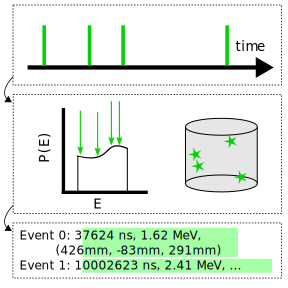
\includegraphics[width=0.49\textwidth]{ch_simulation/singles_flow}
    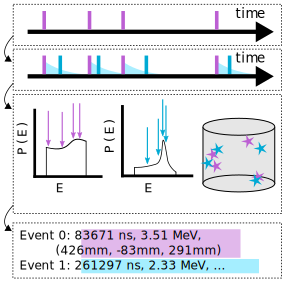
\includegraphics[width=0.49\textwidth]{ch_simulation/correlated_flow}
    \caption{
        Diagram depicting the data stream simulation steps
        for Single events (left) and Correlated events (right).
        The steps are event count and timestamps (top),
        energy and position (middle), and serialization (bottom).
        Different colors represent different event types:
        green, violet and blue represent Single,
        prompt Correlated and delayed Correlated,
        respectively.
        The highlight colors in the serialization phase
        represent the ``truth'' information stored separately.
    }
    \label{fig:my_toymc_flowchart}
\end{figure}


The simulation is based on a core set of event types:
Single, Correlated, and Muon.
Additional event types such as Flasher were added to support specific studies
(see \cref{subsec:toymc_flashers}).
The simulation's configuration allows for customization of the event rate
for each different event type,
and also for multiple variants of the event type.
For example, one type of Correlated event could be configured to represent nH IBDs,
and a second type could be configured to represent nGd IBDs
with a shorter coincidence time, higher delayed energy,
and with the delayed event's position limited to the GdLS (IAV) region of the AD.

\subsection{Types of generated events}

Single events represent uncorrelated signals,
which in Daya Bay were primarily caused by natural radioactive decays in the AD
(\cref{subsec:singles}).
In the simulation, Single events are assigned timestamps
drawn uniformly at random between the time limits given in the configuration,
representing their uncorrelated nature.
The event energies are also drawn uniformly at random
between \SIlist{1;3.5}{\MeV},
and the positions are similarly randomly assigned
within the scintillating volume.
(The energy and position distributions can both be customized
but were left at their defaults for the studies described here.)

Correlated events represent pairs of signals
with a common physical origin, both in position and in time.
IBDs and correlated backgrounds (\cref{sec:correlated_bg})
satisfy these criteria for being modeled by the Correlated event type.
To create the time correlation between prompt and delayed events,
modeled as an exponential distribution,
the simulation first determines the timestamp for a prompt event at random.
Then the coincidence time delay between prompt and delayed events is generated
from an exponential distribution
whose time constant is specified in the simulation configuration.
The prompt and delayed energies are determined independently at random
using uniform distributions specified by the simulation configuration.
The position of the prompt event is chosen at random
within the GdLS or LS volumes (again, as specified by the configuration),
and the delayed position is chosen to be correlated with the prompt position.
Since exact modeling of the position correlations is not crucial,
a simple exponential distribution is used to determine the displacement
in each direction ($x,y,$ and $z$) for these Correlated events.
In the recorded truth information,
prompt and delayed events are assigned separate labels.

Muon events represent signals created by muons traversing
the water pools and ADs (\cref{sec:muonveto}).
For simplicity, each muon is assumed to create a signal
in the inner water pool with a probability of \SI{100}{\percent}.
The rates and energies were chosen to approximately model
the true distributions and rates of muon signals in the near halls (EH1 and EH2).
A portion of the muon signals, \SI{19.95}{\percent},
traverse the AD, depositing an energy chosen at random between
\SIlist{20;2000}{\MeV}.
A smaller subset of the muon signals, \SI{0.05}{\percent},
create particle showers in the AD, depositing an energy chosen at random between
\SIlist{2500;5000}{\MeV}.
The time delay between WP and AD muons is assigned to be \SI{50}{\ns},
chosen since in real data there is a nonzero time offset between WP and AD muons,
but the distribution of time offsets
is not a critical feature of the event selection.
All of the choices of energies and rates are approximations
designed to capture the general behavior of muons at Daya Bay
without adding excessive complexity to the simulation.

%\section{Studies with the simplified Monte Carlo}
%\label{sec:toymc_studies}
\subsection{Study of uncorrelated event rate}

The procedure for determining the uncorrelated event rate
is described in \cref{subsec:singles}.
This process, both the abstract algorithm and the actual software implementation,
was validated using simulated datasets.
The simulation was configured to generate Single (uncorrelated) events
with a rate of \SI{20}{\Hz}
in data files also containing Muon and Correlated events.
The full configuration is listed in \cref{tab:toymc_singles_config}.
%100 simulated data sets were generated,
%each consisting of 300 files containing 10 minutes' worth of data,
%for a total of 50 hours of data per data set.
%This 10-minute structure approximated the file length for near hall data files.
100 simulated data files were generated,
each containing 1000 minutes' worth of data.
The data files were processed using the event selection software
and an empirical rate for uncorrelated events was extracted
for each of the 100 files.
The distribution of measured uncorrelated event rates
is shown in \cref{fig:toymc_singles_dist}.
The mean rate over all 100 data sets
was \SI{19.9966+-0.0022}{\Hz},
which is a bias of \SI{0.017}{\percent} or 2 standard deviations.
This bias was considered acceptable
since the accidentals rate uncertainty
for the actual data set was approximately \SI{0.077}{\percent}.
Thus the simulation was able to confirm that
the event selection software could successfully extract
the uncorrelated event rate with high precision and tolerable bias.

\begin{table}[ht]
    \centering
    \begin{tabular}[t]{llll}
        \hline
        Event type & {Rate [\si{\Hz}]} & Energy [\si{\MeV}] & Coincidence time [\si{\us}]\\
        \hline
        Single & \num{20} & $[\num{1.5}, \num{3}]$ & -\\
        \arrayrulecolor{lightgray}
        \hline
        \multirow{2}{*}{Correlated (nH)}
               & \multirow{2}{*}{\num{0.005}}
               & [\num{0.7}, \num{4}] (prompt)
               & \multirow{2}{*}{\num{150}} \\
               & & [\num{1.9}, \num{2.3}] (delayed) & \\
        \hline
        \multirow{2}{*}{Correlated (nGd)}
               & \multirow{2}{*}{\num{0.0067}}
               & [\num{0.7}, \num{4}] (prompt)
               & \multirow{2}{*}{\num{28}} \\
               & & [\num{7}, \num{9}] (delayed) & \\
        \hline
        Water Pool Muon & \num{200} & - & - \\
        \hline
        AD Muon & \num{39.9} & [\num{20}, \num{2000}] & -\\
        \hline
        Showering Muon & \num{0.1} & [\num{2500}, \num{5000}] & -\\
        \arrayrulecolor{black}
        \hline
    \end{tabular}
    \caption{
        Simulation configuration inputs for the uncorrelated event rate study.
        The rates, energies and coincidence times were simplified
        to allow for faster simulation,
        and no results based on the specific distributions of these quantities
        were used in the final analysis.
    }
    \label{tab:toymc_singles_config}
\end{table}

\begin{figure}
    \centering
    %\includegraphics[width=0.7\textwidth]{ch_simulation/singles_rate_dist}
    \includegraphics[width=0.7\textwidth]{ch_simulation/singles_rate_unbiased_dist}
    \caption{
        Distribution of uncorrelated event rates over 100 simulated data sets.
        The simulation configuration (``truth'') specified a rate of \SI{20}{\Hz}.
        Each data set consists of a single 1000-minute data file.
    }
    \label{fig:toymc_singles_dist}
\end{figure}

\subsection{Study of residual flashers}
\label{subsec:toymc_flashers}

Light emission by PMTs caused a background of single events
known as flashers \cref{sec:flashers}.
The vast majority of flasher events were rejected using an event-by-event veto,
and the remaining flashers were assumed to be accounted for
by the treatment of the accidental background (\cref{sec:acc}).
Certain PMTs were observed to flash with a frequency
of approximately \SI{0.1}{\Hz},
but with the restriction that
the same PMT never flashed twice within $\lesssim$\SI{0.7}{\s}
(see \cref{fig:flasher_anticorr}).
This pattern violated the assumption in the accidental background analysis
that all single events were uncorrelated and governed by Poisson statistics.
A Flasher event type was added to the simulation to test the impact of this deviation.

The Flasher event type had a fixed energy and position
and generated events were assigned fixed, deterministic timestamps \SI{1}{\s} apart
to simulate a maximally-anticorrelated process with no possible time coincidences.
A data sample was generated with only Single events and Flasher events,
and was treated as if the Flasher events passed the existing flasher veto criteria.
The Single events had the same configuration as in \cref{tab:toymc_singles_config},
and the Flasher events were assigned a fixed energy of \SI{2.7}{\MeV}.
The accidental background analysis was performed on this data sample;
after subtracting the accidental background,
the expectation was that 0 correlated events should remain.
\Cref{fig:sim_flasher_prompt_delayed} shows the result of the prompt-delayed spectrum
after subtracting the accidental background
for simulated samples with and without Flasher events \cite{flasher_sim}.
The sample including the Flashers shows
an inaccurate background-subtracted spectrum
due to the synthetic background sample containing unphysical Flasher-Flasher pairs.
In the ``real'' (simulated) data set,
there were no accidental coincidences between residual Flashers by construction,
since the residual Flasher events were generated with \SI{1}{\s} time gaps
between consecutive Flashers.
This simulation was intentionally an extreme configuration,
but it led to the decision to find ways to veto the residual flasher events
rather than attempt to correct for them in other ways.

\begin{figure}
    \centering
    \includegraphics[width=0.73\textwidth]{ch_simulation/flasher_prompt_delayed}
    \caption{
        Accidentals-subtracted prompt vs. delayed energy for simulated data samples
        including only Single events (top) or Single and Flasher events (bottom).
        The Singles-only histogram correctly shows 0 events remaining
        after subtracting the accidental background.
        In the with-Flashers histogram,
        the single energy bin containing (\SI{2.7}{\MeV}, \SI{2.7}{\MeV})
        (the energy of the simulated Flasher events)
        has a negative bin content,
        validating that the Flasher events
        will contaminate the synthetic accidental background,
        form Flasher-Flasher pairs, and cause a distortion to the subtracted spectrum.
        Figure taken from \cite{flasher_sim}.
    }
    \label{fig:sim_flasher_prompt_delayed}
\end{figure}


%A simplified Monte Carlo simulation was developed to model the structure
%of the Daya Bay data stream \cite{dyb_toymc, dyb_toymc_docdb}.
%Rather than simulating the details of physical processes such as scintillation,
%neutron capture, and electronics response,
%the simplified Monte Carlo used parametrized distributions
%to determine the most relevant AD-level observables including the event timestamp
%and reconstructed energy and position.
%This simulation was configured to match various assumptions
%about the Daya Bay data model,
%such as a particular rate of uncorrelated events,
%or the presence or absence of a certain background.
%The resulting output data sets could then be analyzed
%to determine the validity of the analysis
%under the input configuration.
%Data sets could be generated with different assumptions
%about time correlations or position distributions,
%and impact of those assumptions on the final analysis could be assessed.
%However, due to its simplified nature,
%the simulation was not able to provide insights about the distributions themselves.

%A second, more detailed, Monte Carlo simulation was used
%to investigate the detector's response to individual events\todo{cite THU MC}.
%This simulation included detailed tracking of individual energy depositions,
%scintillator response, and particle interactions such as positron annihilation.
%The resulting data sets consisted of detailed information about individual
%simulated IBD events,
%such as the incident \nuebar{} energy, the target volume (LS or GdLS),
%neutron kinetic energy, etc.,
%as well as the reconstructed position and energy
%based on the simulated electronics response.
%This data set could be used to extract efficiencies
%by computing the fraction of simulated events which satisfied
%various analysis cut criteria.

%The detailed simulation produced each event independently,
%and did not attempt to simulate the actual Daya Bay data files
%containing multiple types of events with various time correlations.
%Thus each simulation had a specialized domain,
%and both were necessary to complete the analysis.
%The simplified simulation was able to answer questions about the more complicated
%event selection procedures such as determining the accidental background
%or the \li{} and \he{} contamination (\cref{sec:acc,subsec:li9}),
%and the detailed simulation was able to estimate
%the prompt and delayed energy cut efficiencies (\cref{sec:energy_cuts}).
%The details of the simplified and detailed simulations will be described
%in \cref{sec:toymc,sec:thu_toymc}, respectively.
%A sample of studies that relied on the simulations will be presented
%%in \cref{sec:toymc_studies,sec:thu_toymc_studies}.



%\section{Studies using the detailed Monte Carlo}
%\label{sec:thu_toymc_studies}

%\subsection{Prompt energy efficiency}
%\label{subsec:thu_toymc_prompt}

%The detailed Monte Carlo was used to estimate the prompt energy efficiency,
%the fraction of IBD events whose reconstructed prompt energy
%satisfied the prompt energy criterion of $E > \SI{1.5}{\MeV}$
%(\cref{subsec:prompt_energy}).
%The spectrum of reconstructed energy for the Monte Carlo sample of IBD prompt events
%is shown in \cref{fig:prompt_eff_mc}.
%The prompt energy cut efficiency is the fraction of events in the histogram
%with energy above \SI{1.5}{\mev}.
%\todo[inline]{Fill in details of absolute efficiency determination}

%The AD-uncorrelated uncertainty on the prompt energy efficiency
%was also determined using the simulation.
%Each AD has a slightly different relative energy scale (\cref{subsec:rel_energyscale}),
%resulting in different fractions of IBD prompt events
%being assigned a reconstructed energy above \SI{1.5}{\MeV}.
%The relative energy scale variation was measured to be \SI{+-0.5}{\percent},
%and this effect was reproduced by simply
%scaling the reconstructed energy for each simulated event by \SI{+-0.5}{\percent}.
%The variation in efficiency due to this re-scaling,
%and therefore the AD-uncorrelated relative uncertainty on the prompt energy efficiency,
%was \SI{+-0.1}{\percent}.


\section{The data set toy Monte Carlo}
\label{sec:lbnl_toymc}

An independent toy Monte Carlo was implemented
to generate spectra of reconstructed prompt energy for each AD,
under assumptions of a wide variety of systematic uncertainties,
backgrounds, and reactor parameters.
This simulation was originally \cite{lbnl_toymc,p12e_fitter,p14a_fitter} used to generate covariance matrices for
and validate the performance of
one of the fitter programs for the nGd analysis
\cite[Method A of][]{ngd2016}.
It was used essentially unmodified to validate the fitter for this (nH) analysis
(\cref{ch:analysis}).

The simulation received as input predicted \nuebar{} flux and spectrum data
which were computed \cite{christine_reactor} based on data from the reactor operator
and the models by Huber \cite{reactor_huber}
and Mueller \emph{et al.} \cite{reactor_mueller}.
For each reactor-AD pair, the spectra were updated
based on the configured oscillation parameters
and suppressed by $\nicefrac{1}{L^2}$ due to isotropic emission.
The true \nuebar{} spectrum for IBD interactions was computed
based on the IBD cross section \cite{ibd_xsec,ibd_xsec_note},
number of target protons, and the projected reactor flux.
The detection efficiencies and muon and multiplicity veto efficiencies
were also applied.
A model for the detector response was applied to the true interaction energy
to account for the conversion to positron energy,
energy losses in the IAV,
energy nonlinearities in the scintillator and electronics,
and the energy resolution.
The final simulated energies could be scaled by a fixed factor
to account for the relative energy scale uncertainty.
All of the quantities just mentioned could be configured
to be either known or uncertain, in which case
the relevant values in the simulation would be
adjusted by a configurable random amount
to simulate a systematic uncertainty.
Predicted rates and spectra for background events
were added after the IBD prompt spectra were fully generated.
The backgrounds could be randomly fluctuated to account for
uncertainties in their rates and spectra.
Lastly, the number of events in each bin of reconstructed energy
could optionally be fluctuated to account for statistical uncertainty.
\Cref{fig:lbnl_toymc_flowchart} shows the above steps as a flowchart.
\todo[inline]{Finish LBNL ToyMC section}

\begin{figure}
    \includegraphics[width=0.6\textwidth]{ch_simulation/lbnl_toymc_flowchart}
    \caption{
        Steps to simulate the prompt reconstructed spectra
        at each AD.
        Figure taken from \cite{lbnl_toymc}.
    }
    \label{fig:lbnl_toymc_flowchart}
\end{figure}

%Hundreds of thousands of simulated data sets were generated
%using this simulation
%in order to validate the fitter for this analysis.
%The simulation's configuration was modified
%to allow for the ability to disable fluctuations
%independently at the near sites and far site,
%since the $\chi^2$ expression for the fit
%treated the near and far sites differently.
